%%%%%%%%%%%%%%%%%%%%%%%%%%%%%%%%%%%%%%%%%
% Beamer Presentation
% LaTeX Template
% Version 1.0 (10/11/12)
%
% This template has been downloaded from:
% http://www.LaTeXTemplates.com
%
% License:
% CC BY-NC-SA 3.0 (http://creativecommons.org/licenses/by-nc-sa/3.0/)
%
%%%%%%%%%%%%%%%%%%%%%%%%%%%%%%%%%%%%%%%%%

%----------------------------------------------------------------------------------------
%	PACKAGES AND THEMES
%----------------------------------------------------------------------------------------

\documentclass{beamer}

\mode<presentation> {

% The Beamer class comes with a number of default slide themes
% which change the colors and layouts of slides. Below this is a list
% of all the themes, uncomment each in turn to see what they look like.

% \usetheme{default}
% \usetheme{AnnArbor}
% \usetheme{Antibes}
% \usetheme{Bergen}
% \usetheme{Berkeley}
% \usetheme{Berlin}
\usetheme{Boadilla}
% \usetheme{CambridgeUS}
% \usetheme{Copenhagen}
% \usetheme{Darmstadt}
% \usetheme{Dresden}
% \usetheme{Frankfurt}
% \usetheme{Goettingen}
% \usetheme{Hannover}
% \usetheme{Ilmenau}
% \usetheme{JuanLesPins}
% \usetheme{Luebeck}
% \usetheme{Madrid}
% \usetheme{Malmoe}
% \usetheme{Marburg}
% \usetheme{Montpellier}
% \usetheme{PaloAlto}
% \usetheme{Pittsburgh}
% \usetheme{Rochester}
% \usetheme{Singapore}
% \usetheme{Szeged}
% \usetheme{Warsaw}

% As well as themes, the Beamer class has a number of color themes
% for any slide theme. Uncomment each of these in turn to see how it
% changes the colors of your current slide theme.

%\usecolortheme{albatross}
%\usecolortheme{beaver}
%\usecolortheme{beetle}
%\usecolortheme{crane}
%\usecolortheme{dolphin}
%\usecolortheme{dove}
%\usecolortheme{fly}
%\usecolortheme{lily}
%\usecolortheme{orchid}
%\usecolortheme{rose}
%\usecolortheme{seagull}
%\usecolortheme{seahorse}
%\usecolortheme{whale}
%\usecolortheme{wolverine}

%\setbeamertemplate{footline} % To remove the footer line in all slides uncomment this line
%\setbeamertemplate{footline}[page number] % To replace the footer line in all slides with a simple slide count uncomment this line

%\setbeamertemplate{navigation symbols}{} % To remove the navigation symbols from the bottom of all slides uncomment this line
}

\usepackage{booktabs} % Allows the use of \toprule, \midrule and \bottomrule in tables
\usepackage{graphicx}
\usepackage{subcaption}
%----------------------------------------------------------------------------------------
%	TITLE PAGE
%----------------------------------------------------------------------------------------

\title[\tiny{Response in Discrete Space GANs}]{Response Generation in Discrete Space Using GANs} % The short title appears at the bottom of every slide, the full title is only on the title page

\author[M. Zhao et F. Mi]{\underline{Mengjie Zhao}  \and Fei Mi } % Your name
\institute[] % Your institution as it will appear on the bottom of every slide, may be shorthand to save space
{
\footnotesize{Artificial Intelligence Laboratory (LIA)}
\date{\today}
\\\medskip
\medskip
\medskip
\medskip
\medskip
\medskip
% \footnotesize{\'Ecole polytechnique f\'ed\'erale de Lausanne} \\ % Your institution for the title page
\medskip
% \textit{john@smith.com} % Your email address
\vspace{-1cm}
\begin{figure}
\includegraphics[width=0.2\linewidth]{imgs/epfl1.eps}
\end{figure}
}

 % Date, can be changed to a custom date

\begin{document}
\begin{frame}
\titlepage % Print the title page as the first slide
\end{frame}

\begin{frame}
\frametitle{Overview} % Table of contents slide, comment this block out to remove it
\tableofcontents % Throughout your presentation, if you choose to use \section{} and \subsection{} commands, these will automatically be printed on this slide as an overview of your presentation
\end{frame}

%----------------------------------------------------------------------------------------
%	PRESENTATION SLIDES
%----------------------------------------------------------------------------------------

%------------------------------------------------
\section{A quick reminder of GANs} % Sections can be created in order to organize your presentation into discrete blocks, all sections and subsections are automatically printed in the table of contents as an overview of the talk
%------------------------------------------------

\begin{frame}
\frametitle{Application of GAN}
\begin{figure}
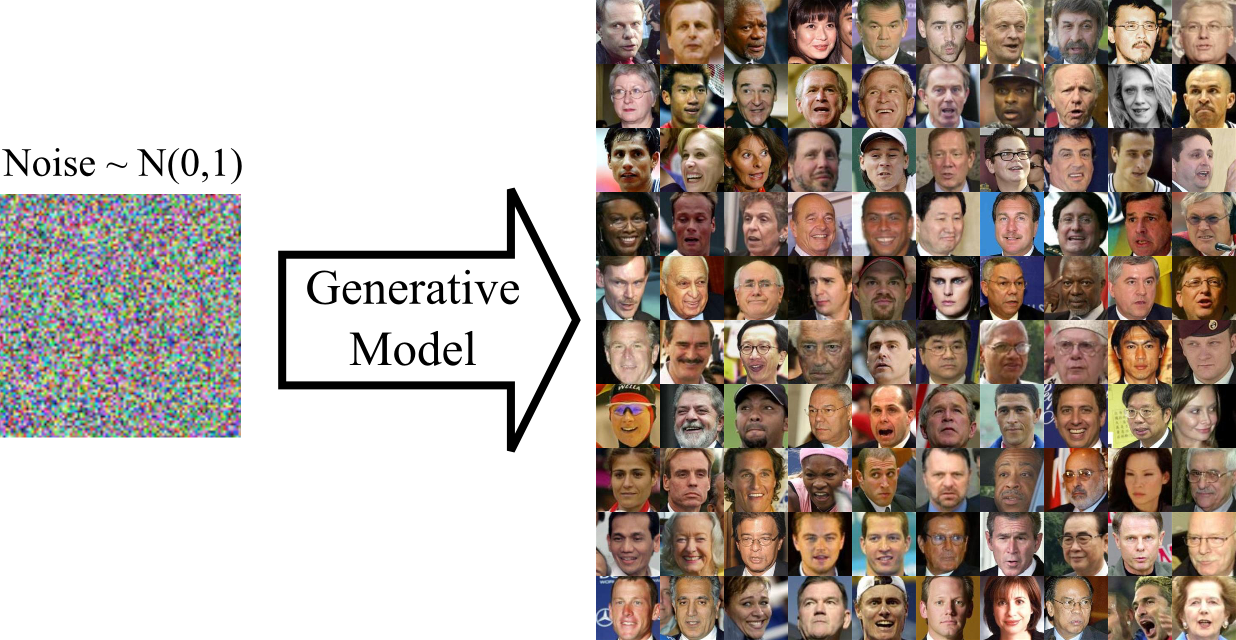
\includegraphics[width=0.8\linewidth]{imgs/w1_g_model.png}
\end{figure}
\hspace{7cm}\tiny{src: http://torch.ch/blog/2015/11/13/gan.html}
\end{frame}


%------------------------------------------------

%------------------------------------------------

\begin{frame}
\frametitle{Performance on images (3-conv-layer CNN)}
\begin{figure}[!htb]
\minipage{0.3\textwidth}
  \includegraphics[width=\linewidth]{imgs/1_face.png}
  \caption*{Noise}\label{fig:awesome_image1}
\endminipage\hfill
\minipage{0.3\textwidth}
  \includegraphics[width=\linewidth]{imgs/2_face.png}
  \caption*{Epoch 1}\label{fig:awesome_image2}
\endminipage\hfill
\minipage{0.3\textwidth}%
  \includegraphics[width=\linewidth]{imgs/3_face.png}
  \caption*{Epoch 3}\label{fig:awesome_image3}
\endminipage
\end{figure}
\hspace{7cm}\tiny\emph{Dataset: Labeled Faces in the Wild Home, UMass}
\end{frame}

%------------------------------------------------

%------------------------------------------------
\begin{frame}
\frametitle{Apply GAN on text}
\begin{itemize}
\item Training the model 
  \begin{itemize}
    \item Training on continuous space
    \item Using \textbf{policy iteration}
  \end{itemize} 
\item Two major types of applications
	\begin{itemize}
		\item Text generation
		\item Response and dialog generation

	\end{itemize}
\end{itemize}
\end{frame}

%------------------------------------------------
\begin{frame}
\frametitle{Overview} 
\tableofcontents 
\end{frame}
%------------------------------------------------

%------------------------------------------------
\section{Our current framework} 
%------------------------------------------------

\begin{frame}
\frametitle{Our current framework in response generation}
\begin{figure}
\centering
\includegraphics[width=\linewidth]{imgs/v2.eps}
\end{figure}
\end{frame}

%------------------------------------------------
%------------------------------------------------
\begin{frame}
\frametitle{The encoder-decoder model}
\begin{itemize}
\item Taking sequences as input and generates sequence as output:
\begin{figure}
\centering
\hspace{-1cm}\includegraphics[width=0.85\linewidth]{imgs/en-de.png}
\end{figure}
\hspace{9cm}\tiny{(C. Olah 2015)}
\end{itemize}
\begin{itemize}
\item Sample results (TBBT dataset):
\begin{itemize}
\item \emph{what is your name ? -- my name is siri .}
\item \emph{do you know switzerland ? -- oh , of course .}
\item \emph{i think you are correct . -- so why are you saying that ?}
\item \emph{can you drive me home ? -- uh , sure .}
\end{itemize}
\end{itemize}
\end{frame}
%------------------------------------------------
%------------------------------------------------
\begin{frame}
\frametitle{Convolution fusion - old proposal}
A': The representation of an answer consisting of time dependency words

  \begin{figure}
      \centering
      \hspace{-1cm}\includegraphics[width=0.75\linewidth]{imgs/idea}
  \end{figure}
\end{frame}
%------------------------------------------------

%------------------------------------------------
\begin{frame}
\frametitle{Fusing in another latent space}
\begin{itemize}
\item For each candidate answer from beam search, we express its embedding in another latent space:
  \begin{figure}
      \centering
      \hspace{-1cm}\includegraphics[width=0.85\linewidth, height=0.65\linewidth]{imgs/fuse}
  \end{figure}
\end{itemize}
\end{frame}
%------------------------------------------------

%------------------------------------------------
\begin{frame}
\frametitle{Fusing in another latent space}
\begin{itemize}
\item Take weighted average of the new latent expressions of all candidates from beam search:
      \begin{itemize}
      \item Weights are set based on score of each candidates from beam search.
      \item Trainable weights.
      \end{itemize}
      \vspace{.4cm}
\item Start adversarial training:
      \begin{itemize}
      \item The new fused expression is initial state of the LSTM in SeqGAN.
      \item Use the same embedding from the encoder-decoder model.
      \end{itemize}
\end{itemize}
\end{frame}
%------------------------------------------------

\begin{frame}
\frametitle{Major drawbacks of the proposed framework}
\begin{figure}
\centering
\includegraphics[width=\linewidth]{imgs/v2.eps}
\end{figure}
\begin{itemize}
\item Not end-to-end due to the beam search operation.
\item More parameters introduced due to the increase of model depth.
\item Need to check if the gradient could be backpropagated to update parameters in the fusing operation. 
\end{itemize}
\end{frame}

%------------------------------------------------
\begin{frame}
\frametitle{Similar framework for dialog generation (Li et al. 2017)}
\begin{itemize}
\item Use \emph{seq2seq} model as a generator to generate dialog
\item Discriminator decides the source of the dialog
\begin{itemize}
\item Using Monte Carlo search to score sentences.
\item Make the discriminator can score both full and partial sentences.
\end{itemize}
\end{itemize}
\end{frame}
%------------------------------------------------

%------------------------------------------------
\begin{frame}
\frametitle{Overview} % Table of contents slide, comment this block out to remove it
\tableofcontents % Throughout your presentation, if you choose to use \section{} and \subsection{} commands, these will automatically be printed on this slide as an overview of your presentation
\end{frame}
%------------------------------------------------


%------------------------------------------------
\section{Rate of progress}
%------------------------------------------------
\begin{frame}
\frametitle{Rate of progress}
\begin{figure}
\centering
\includegraphics[width=\linewidth]{imgs/gantt2}
\end{figure}
\end{frame}

%------------------------------------------------
\section{Conclusion}
%------------------------------------------------
\begin{frame}
\frametitle{Conclusion}
\begin{itemize}
% \item Adversarial training for generative models
\item Individual component of the proposed model is implemented.
\item Need to check if the gradients could be backpropagated to update parameters in the fusion operation.
\item Determine if the fusion could improve model performance.
\item Try other generative models to make the whole framework end-to-end.

\end{itemize}
\end{frame}

%------------------------------------------------

%------------------------------------------------
\begin{frame}
\vspace{3cm}
\Huge{\centerline{That's it!}}
\begin{figure}
\hspace{-7cm}
\vspace{-1cm}
\includegraphics[width=0.3\linewidth]{imgs/bt2.jpg}
\end{figure}
\end{frame}
%---------------------------------------------------

\begin{frame}
\frametitle{References}
\footnotesize{
\begin{thebibliography}{99} % Beamer does not support BibTeX so references must be inserted manually as below

\bibitem[C, Olah]{p1} C. Olah (2015)
\newblock Computer, respond to this email.
\newblock \emph{Google Research Blog}

\bibitem[Yu et al]{p1} Yu et al. (2017)
\newblock SeqGAN: Sequence Generative Adversarial Nets with Policy Gradient 
\newblock \emph{AAAI 17}

\bibitem[Li et. al.]{p1} Li et al. (2017)
\newblock Adversarial Learning for Neural Dialogue Generation
\newblock \emph{arXiv:1701.06547}

\end{thebibliography}
}
\end{frame}

%-------------------------------------

%------------------------------------------------
\begin{frame}
\frametitle{Appendix}
\begin{itemize}
\item BLEU (bilingual evaluation understudy):
	\begin{itemize}
 		\item the closer a machine translation is to a professional human translation, the better it is
 		\item evaluating the quality of text which has been machine-translated from one natural language to another. 
 	\end{itemize}
 \item GitHub: @joemzhao
 \item Likelihood:
		 \begin{figure}
			\centering
			\includegraphics[width=0.7\linewidth]{imgs/likelihood}
		\end{figure}
\end{itemize}
\end{frame}
%---------------------------------------------------

%------------------------------------------------
\begin{frame}
\frametitle{Appendix}
\begin{itemize}
\item SeqGAN 
\begin{itemize}
		\item Generator LSTM maximize the expected rewards
		\item Discriminator TextCNN minimize cross entropy
\end{itemize}
\end{itemize}
\end{frame}
%---------------------------------------------------

\end{document}